%!TEX root = ../my_thesis.tex
\section{Decay-time resolution}
\label{sec:time:resol}

The decay-time resolution is determined from a sample of fake $\Bz$ candidates formed from a prompt \Dpm~candidate combined with a track originating from the PV. This is sample is referred to as ``\Dpm+track''. The candidates are taken from the \texttt{B02DKLTUBD2HHH} stripping line. They are subjected to the same offline selection as that of the signal sample without a BDT cut and with two additional requirements: a single reconstructed PV per event is required in order to reduce wrong PV associations, and the \Dpm~IP $\chi^{2}$ with respect to the PV is required to be less than 9 to reduce the $\Dmp$ contribution from $\Bz$ decays. The combined stripping and offline selection yields $51\,053$ candidates. True \Dpm+track candidates are unfolded from combinatorial background and nonresonant decays by means of \emph{sWeights} computed via a fit to the $\Kpm\pimp\pimp$ invariant mass distribution.

\subsection{Companion track momentum reweighting}

The decay time resolution is found to be dependent upon the companion track \pt~which is considerably lower on average for the \Dpm+track candidates than it is for genuine \Bz\to\Dpm\pimp~signal. This is corrected for by reweighting the prompt sample to have the same $\ln(\pt)$ distribution as that of the $\Bz\to\Dmp\pipm$ signal. The logarithm is taken to compress the high-\pt~tails, and a binning scheme is chosen to have an equal number of signal events per bin. The $\ln(\pt)$ spectra for signal, prompt, and reweighted prompt candidates is shown in Fig.~\ref{fig:reweights}. By following the steps described in Sec.~\ref{sec:resolution}, prior to reweighting the average proper time resolution is determined to be $\sim71$\fs, and after reweighting the resolution is found to be consistent with the value of $54~\rm fs$ that was obtained in other $B$ meson time-dependent analyses~\cite{LHCB-PAPER-2014-051}.  
\begin{figure}[t]
	\begin{center}
		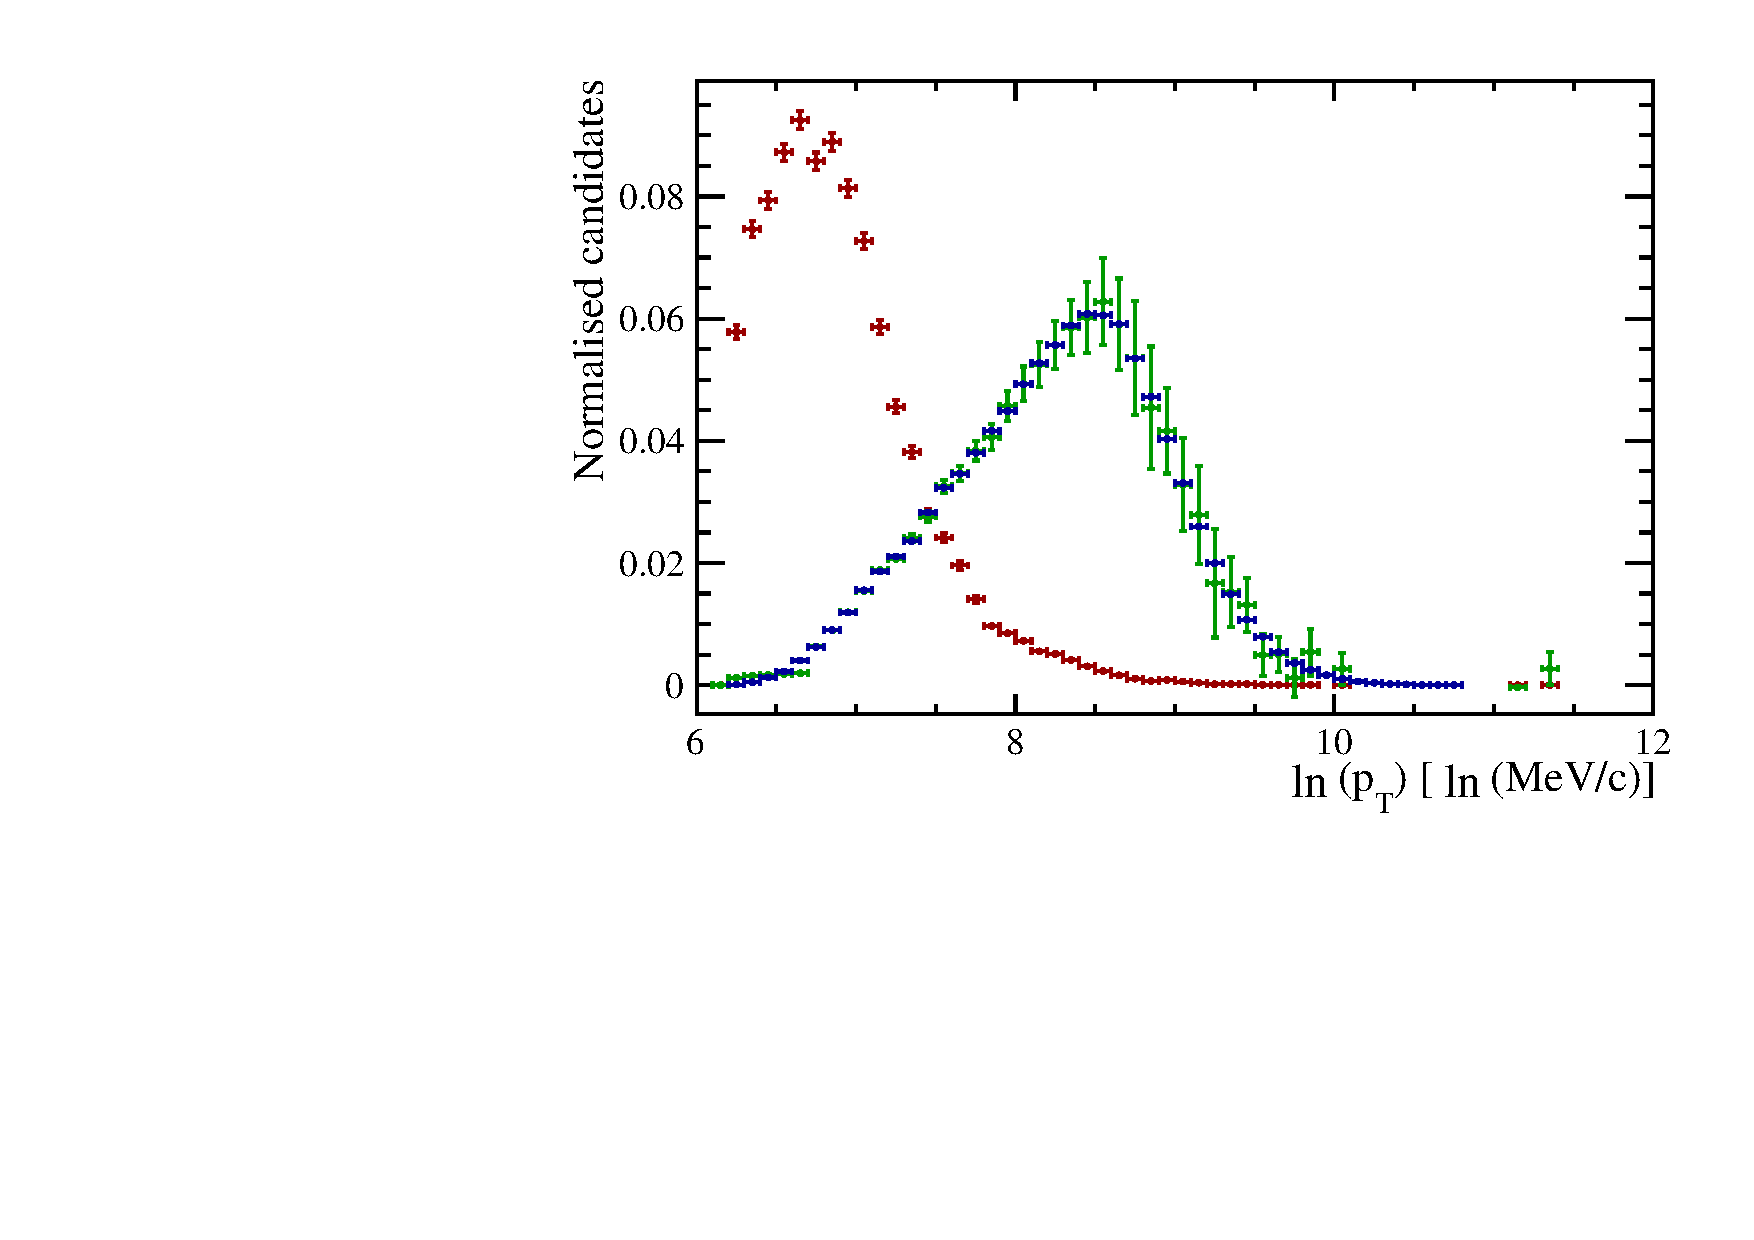
\includegraphics[width=0.60\linewidth]{05DecaytimeFit/figs/resolution/reweighting.pdf}
	\end{center}
        \vspace{-2mm}
			      \caption{Normalised $\ln(\pt)$ distributions of \emph{sWeighted} \Bz\to\Dpm\pimp signal (blue), prompt \Dpm+track before reweighting (red) and after reweighting (green).
				  \label{fig:reweights}}
\end{figure}

\subsection{Resolution determination from decay-time error parameterisation}
\label{sec:resolution}

In order to study potential second order corrections to the decay-time error distribution, fits to the decay-time distribution of the $\Dpm$+track sample in bins of the per-event decay time error are performed. The decay-time error is obtained from DTF by propagating the uncertainty on the $\Bz$ four-momentum. The binning scheme is chosen such that the sum of the \emph{sWeights} associated to $\Dpm$+track candidates in each bin is equal. The fit is similar to that used to determine the resolution in Ref.~\cite{LHCb-PAPER-2014-059}, consisting of three components: a delta function convolved with a Gaussian resolution function accounts for the genuine prompt \Dpm+track component; a pair of exponential functions convolved with the same Gaussian function accounts for signal candidates coming from $b$-hadron decays, and a Gaussian function with a large width accounts for wrong-PV associated backgrounds. The time constant of the exponentials and the mean of the wrong-PV component are fixed from a global fit to the sample, while the mean and width of the resolution, the width of the wrong-PV component and the relative fractions of the prompt, wrong-PV and from-$b$ components are all free parameters in the fits to each decay-time error bin. A likelihood fit is performed in 20 bins of the decay-time error from which the measured resolution $\left<\sigma\right>_{i}$ is determined. The results of these fits are presented in Table~\ref{tab:resPedtefit}, and a representative fit is shown in Fig.~\ref{fig:resPedte}. A $\chi^{2}$ fit is performed to the obtained values of the per-bin average error and resolution of the form:
\begin{equation}
	\left<\sigma\right>_{i} = \left<\sigma\right> + p_{1} \left(\left<\delta\right>_{i} - \left<\delta\right>\right) + p_{2} \left(\left<\delta\right>_{i} - \left<\delta\right>\right)^{2}
\end{equation}
where $\left<\delta\right>$ is the average per-event decay time error of the whole (unbinned) sample, while $\left<\delta\right>_{i}$ is the average per-event decay time error in each bin. In the prompt \Dpm+track sample $\left<\delta\right>$ is determined to be $0.0307\pm0.0097$ ps, in good agreement with the \emph{sWeighted} $\Bz\to\Dmp\pipm$ signal sample value of $0.034\pm0.011$ ps. The fit determines the average resolution, $\left<\sigma\right>$, in addition to the trend. This fit is shown in Fig.~\ref{fig:resPedte}, the result of which is presented in Table~\ref{tab:resPedtecalibFit}. The global average resolution is determined from this fit to be $\left<\sigma\right>=0.05491\pm 0.00038$ ps. The procedure is found to be stable and yields compatible results with fits to 10 bins ($ 0.05523\pm 0.00041$ ps) and 30 bins ($0.05464\pm 0.00037$ ps). 

\begin{figure}[tbp]
	\begin{center}
			 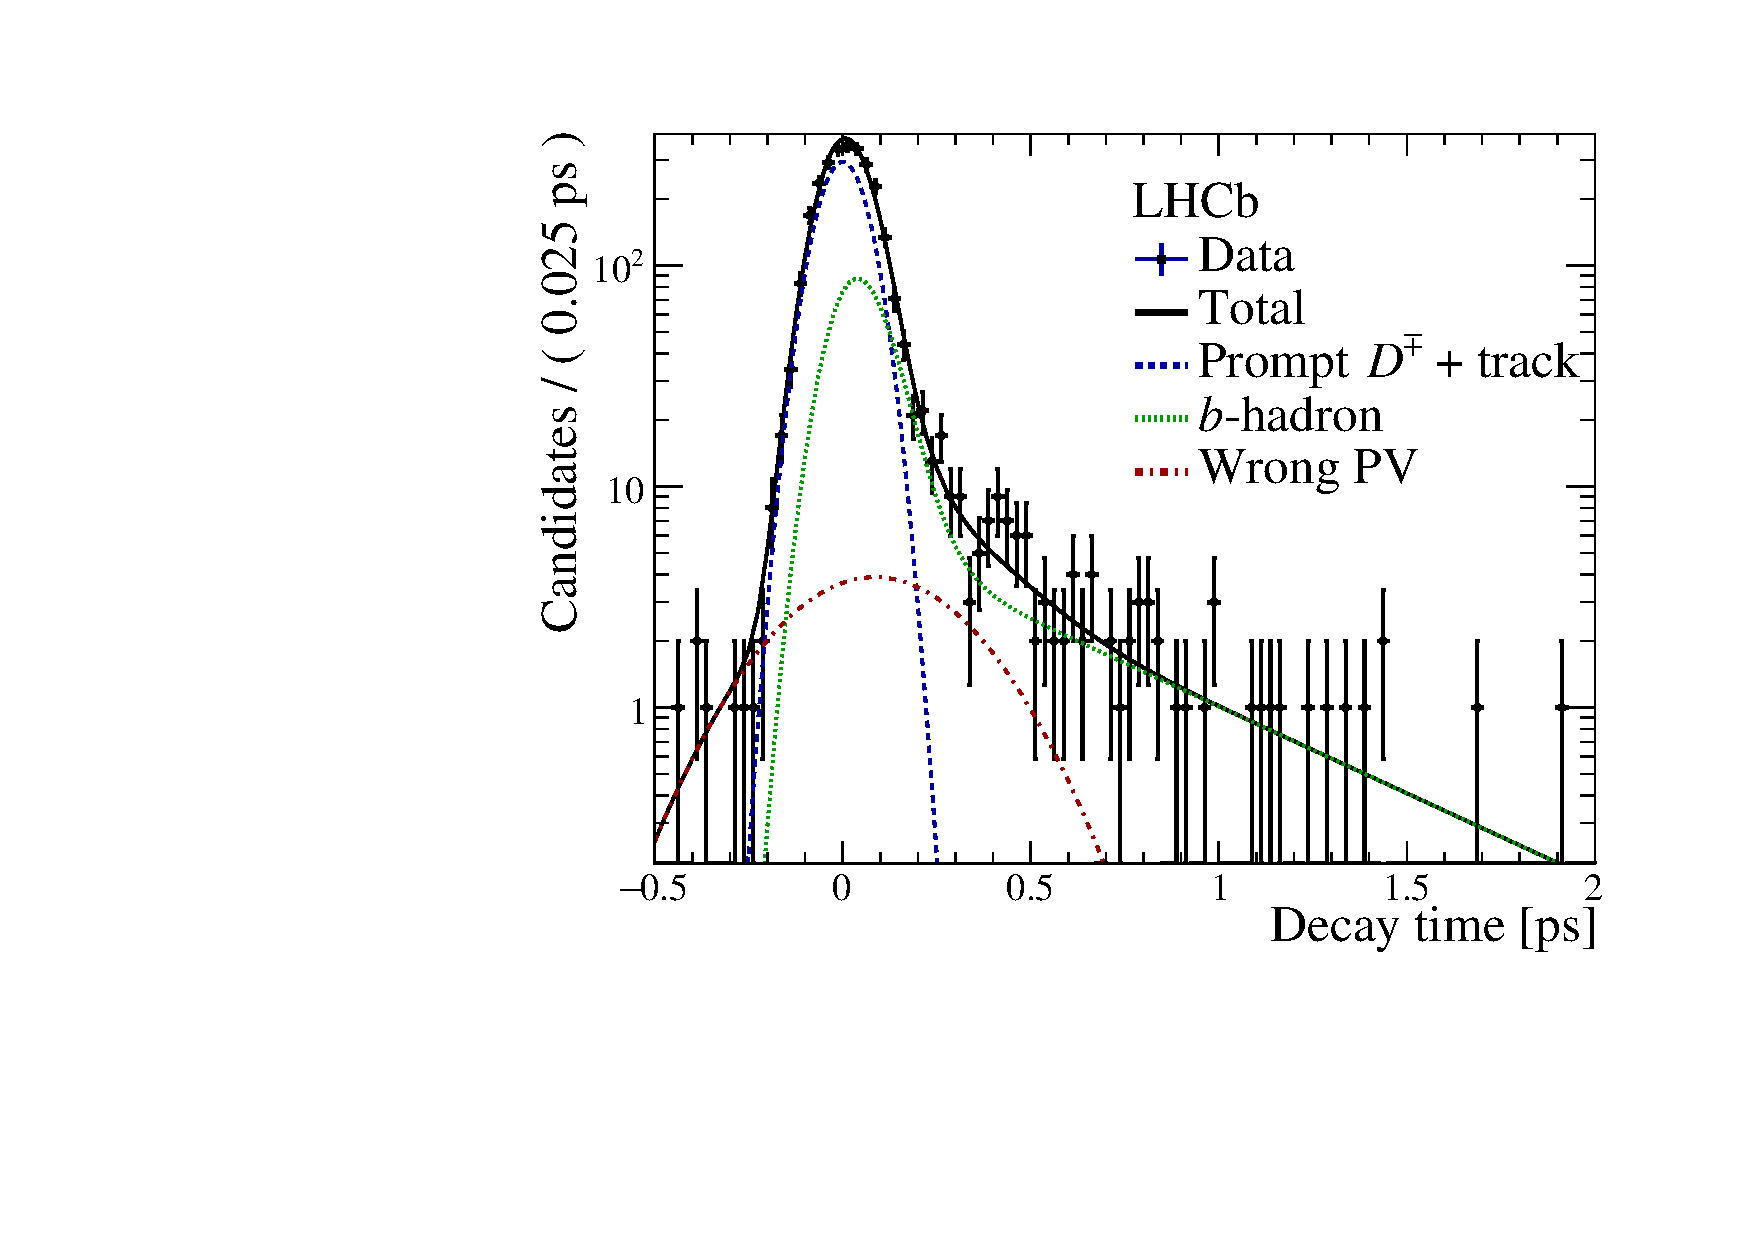
\includegraphics[width=0.49\linewidth]{05DecaytimeFit/figs/resolution/resolution_promptDtimefit_15bin_log_plot.pdf}
			 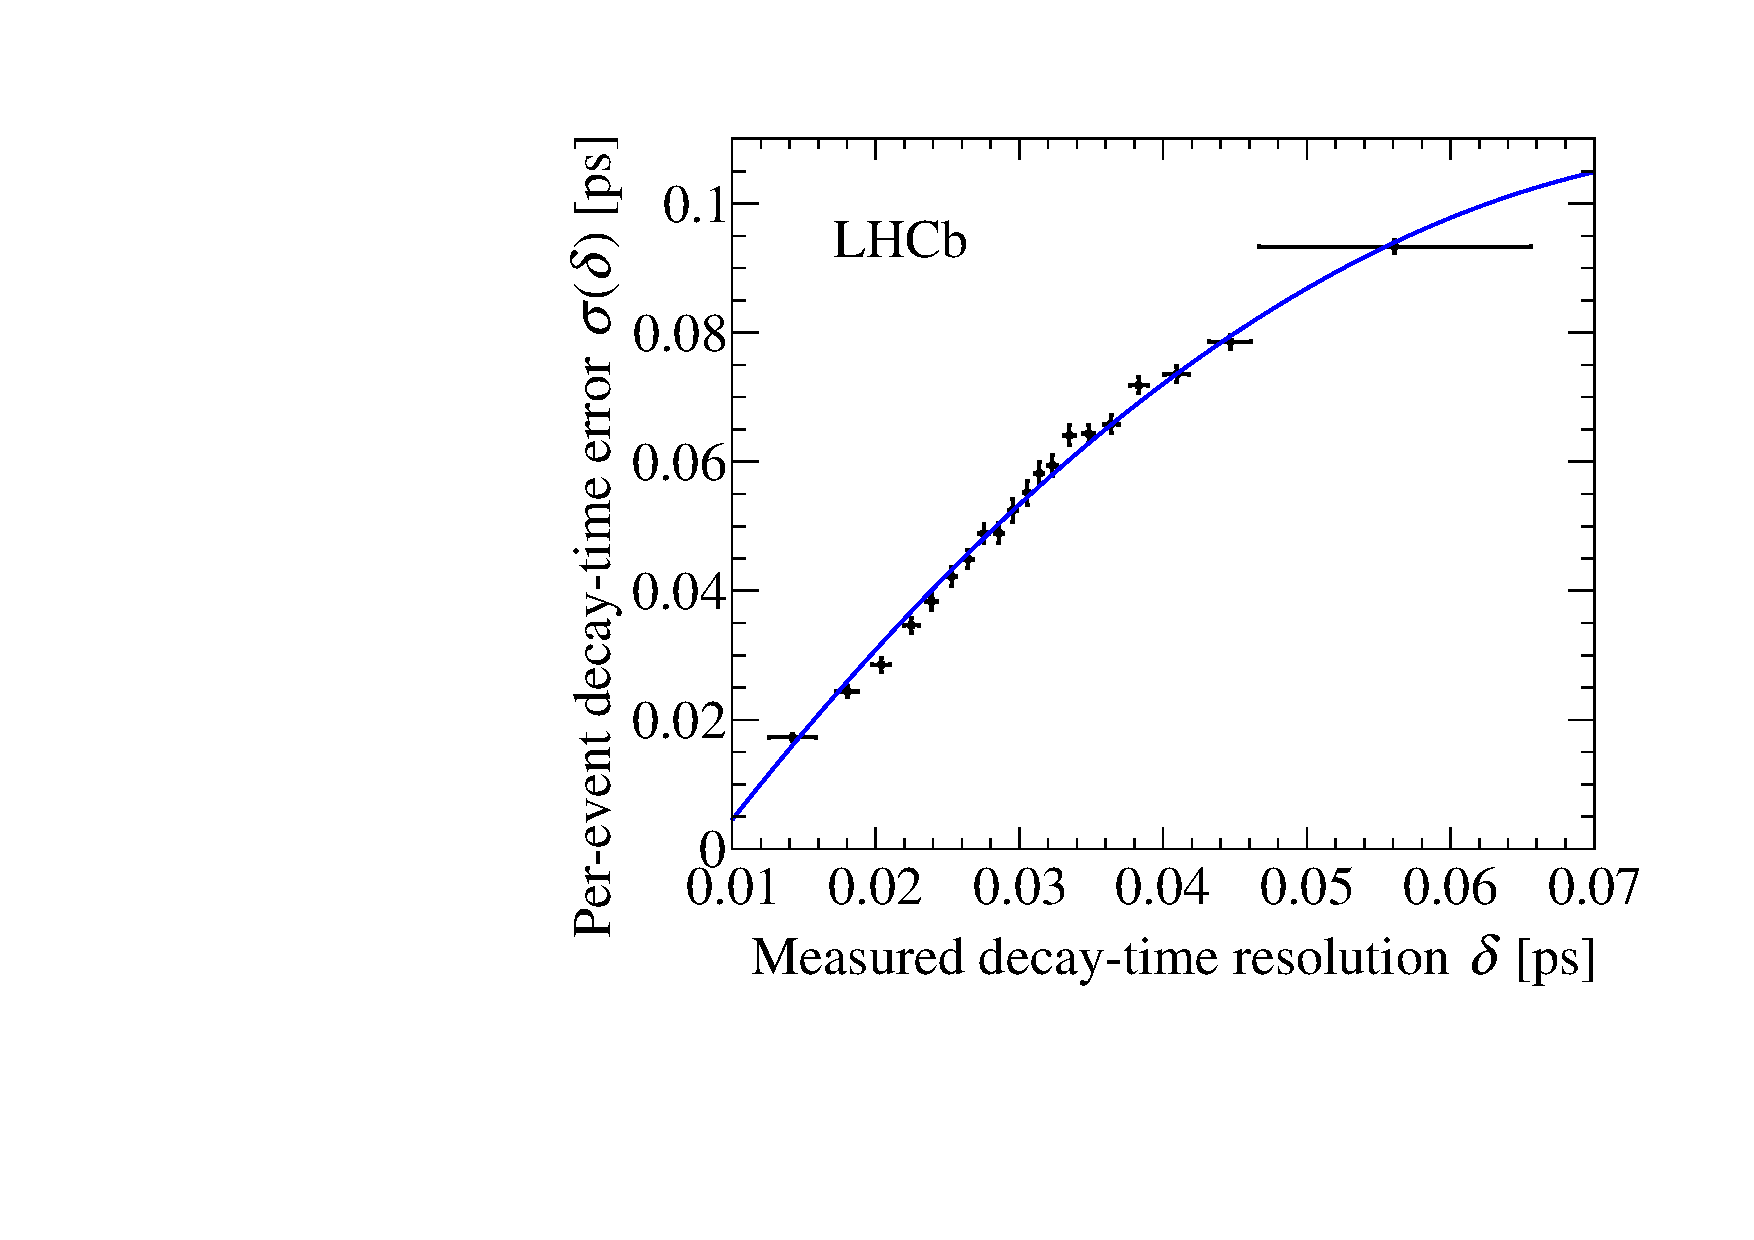
\includegraphics[width=0.49\linewidth]{05DecaytimeFit/figs/resolution/resolution_pedtecalibpdf_pedtecalib_lin_plot.pdf}	
	\end{center}
        \vspace{-2mm}
			      \caption{Left: \pt-corrected and background-subtracted decay-time distribution of the $\Dpm$+track sample for the 15th bin ($[0.0341,0.0355]~\rm ps$) in per-event decay time error. The fit result is overlaid as the black solid curve: the wrong-PV, from-$b$, and prompt components are shown as the red dot-dashed, green dotted, and blue dashed curves, respectively. The numerical results are presented in Table~\ref{tab:resPedtefit}. Right: measured resolution as a function of the average per-event decay time error determined from fits to the decay time in bins of decay time error. The horizontal bars are the standard deviation of the average per-event decay time error in each bin. The overlaid fit is described in the text.
				  \label{fig:resPedte}}
\end{figure}
\begin{table}[tbp]
	\centering
	\caption{Measured resolution $\left<\sigma\right>_{i}$ obtained from a fit to the \pt~corrected \emph{sPlot} of the decay-time distribution in bins of per-event decay-time error, $\delta$, for prompt \Dpm+track signal. The average per-event decay time error $\left<\delta\right>_{i}$ in each bin is also reported.
	\label{tab:resPedtefit}
	}
	\begin{tabular}{llcc}
		\toprule
		Bin $i$& lower edge & $\left<\delta\right>_{i}$ & $\left<\sigma\right>_{i}$ \\
		\midrule
		 0       &       0.01    &       $ 0.0142\pm 0.0016$     &       $ 0.01731\pm 0.00053$   \\
		  1       &       0.0165376       &       $ 0.01801\pm 0.00075$   &       $ 0.02439\pm 0.00089$   \\
		    2       &       0.0192247       &       $ 0.02038\pm 0.00063$   &       $ 0.0286\pm 0.0011$     \\
		    3       &       0.0214493       &       $ 0.02248\pm 0.00052$   &       $ 0.0347\pm 0.0011$     \\
		    4       &       0.0232264       &       $ 0.02388\pm 0.00036$   &       $ 0.0384\pm 0.0013$     \\
		    5       &       0.0245968       &       $ 0.02528\pm 0.00033$   &       $ 0.0422\pm 0.0014$     \\
		    6       &       0.0257605       &       $ 0.02641\pm 0.00034$   &       $ 0.0449\pm 0.0014$     \\
		    7       &       0.0269093       &       $ 0.02753\pm 0.00033$   &       $ 0.0489\pm 0.0015$     \\
		    8       &       0.0280345       &       $ 0.02857\pm 0.00028$   &       $ 0.0489\pm 0.0015$     \\
		    9       &       0.0290414       &       $ 0.02955\pm 0.00030$   &       $ 0.0525\pm 0.0018$     \\
		    10      &       0.0301189       &       $ 0.03054\pm 0.00024$   &       $ 0.0552\pm 0.0019$     \\
		    11      &       0.0309259       &       $ 0.03138\pm 0.00027$   &       $ 0.0582\pm 0.0017$     \\
		    12      &       0.0318409       &       $ 0.03229\pm 0.00032$   &       $ 0.0594\pm 0.0016$     \\
		    13      &       0.0328907       &       $ 0.03347\pm 0.00036$   &       $ 0.0641\pm 0.0015$     \\
		    14      &       0.0341106       &       $ 0.03482\pm 0.00039$   &       $ 0.0643\pm 0.0014$     \\
		    15      &       0.0354999       &       $ 0.03638\pm 0.00052$   &       $ 0.0658\pm 0.0014$     \\
		    16      &       0.0372226       &       $ 0.03830\pm 0.00063$   &       $ 0.0719\pm 0.0012$     \\
		    17      &       0.0395386       &       $ 0.04096\pm 0.00086$   &       $ 0.0736\pm 0.0012$     \\
		    18      &       0.0424521       &       $ 0.0447\pm 0.0014$     &       $ 0.0786\pm 0.0011$     \\
		    19      &       0.0473915       &       $ 0.0561\pm 0.0095$     &       $ 0.0933\pm 0.0010$     \\


		\bottomrule
	\end{tabular}
\end{table}

\begin{table}[tbp]
	\centering
	\caption{Average per-event decay-time error $\left<\delta\right>$, and resolution parameters $p_1$, $p_2$ and $\left<\sigma\right>$ obtained from a fit to the per-bin decay time error.
	\label{tab:resPedtecalibFit}
	}
	\begin{tabular}{lcccl}
		\toprule
		Parameter & Result \\
		\midrule
		$\left<\delta\right>$ & $ 0.0307$&$\pm$&$ 0.0097 $& ps\\
		$p_{1}$ & $ 2.031$&$\pm$&$ 0.022$ &\\
		$p_{2}$ & $ -19.30$&$\pm$&$ 1.6$& $\rm ps^{-1}$ \\
		$\left<\sigma\right>$ & $ 0.05491$&$\pm$&$ 0.00038$ & ps \\ 
		\bottomrule
	\end{tabular}
\end{table}

This method, which accounts for second-order corrections to the decay time error, is used to define the width of a single Gaussian in the decay time fit to data, $\mathcal{R}(t-t')=G(t-t',\left<\sigma\right>)$, with $\left<\sigma\right> = 0.05491\pm 0.00038$ ps. The uncertainty quoted here is statistical.  Systematic uncertainties will be considered in Sec.~\ref{sec:syst_toys_resolution}. 

